% 若编译失败，且生成 .synctex(busy) 辅助文件，可能有两个原因：
% 1. 需要插入的图片不存在：Ctrl + F 搜索 'figure' 将这些代码注释/删除掉即可
% 2. 路径/文件名含中文或空格：更改路径/文件名即可

% --------------------- 文章宏包及相关设置 --------------------- %
% >> ------------------ 文章宏包及相关设置 ------------------ << %
% 设定文章类型与编码格式
\documentclass[UTF8]{article}		
\input{../.config/config_for_MCPExperiment.tex}



%%%%%%%%%%%%%%%%%%%%%%%%%%%%%%%%%%%%%%%%%%%%%%%%%%%%%%%%%%%%%%%%
% 仅需修改页眉、实验名称、实验日期
%%%%%%%%%%%%%%%%%%%%%%%%%%%%%%%%%%%%%%%%%%%%%%%%%%%%%%%%%%%%%%%%


%%%%%%%%%%%%%%%%%% 1. 修改页眉内容 %%%%%%%%%%%%%%%%%%
\rhead{MCP-05 数模转换实验 (2025.12.15, 徐睿琳)}

% 开始编辑文章
\begin{document}
\begin{center}\large
    \vspace*{-0.8cm}
    \noindent{\huge\bfseries《\ \ 微\ \ 机\ \ 原\ \ 理\ \ 实\ \ 验\ \ \ 》\ \ 实\ \ 验\ \ 报\ \ 告 }
    \\\vspace{0.1cm}
    \noindent{
    {\bfseries 
%
%%%%%%%%%%%%%%%%%% 2. 修改实验名称 %%%%%%%%%%%%%%%%%%
    实验名称：\uline{\hspace{2.2cm} 数模转换实验 \hspace{2.2cm}}
%
    }\hspace{0.4cm}
    指导教师：\uline{\hspace{0.8cm}肖山林     \hspace{0.8cm}}
    }
    \\\vspace{0.1cm}
    \noindent
    {
    姓名：\uline{\,\,\,徐睿琳\,\,\,}\hspace{0.2cm}
    学号：\uline{\,\,\,{ 23342107}\,\,\,}\hspace{0.2cm}
    专业/班级：\uline{\,\,\,{微电子/三班}\,\,\,}\hspace{0.2cm}
    分组序号：\uline{\,\,\,{A412-A05}\,\,\,}
    }
    \\\vspace{0.1cm}
    \noindent{
%
%%%%%%%%%%%%%%%%%% 3. 修改实验日期 %%%%%%%%%%%%%%%%%%
    实验日期：\uline{\,\,{2025.12.15}\,\,}\hspace{0.2cm}
%
    实验地点：\uline{\,\,\,教学楼{ A412}\,\,\,}\hspace{0.2cm}
    是否调课/补课：\uline{\hspace{0.26cm}否 \hspace{0.26cm}}\hspace{0.2cm}
    成绩：\uline{\hspace{2cm}}
    }
\end{center}
\vspace{-0.4cm}
\noindent\rule{\textwidth}{0.075em}   % 分割线
\vspace{-1.0cm}

% 生成目录
\setcounter{tocdepth}{3}  % 目录深度为 2（不显示 subsubsection）
\noindent\tableofcontents\thispagestyle{fancy}   % 显示页码、页眉等

% ------------------------ 文章信息区 ------------------------ %
% ------------------------ 文章信息区 ------------------------ %



%%%%%%%%%%%%%%%%%%%%%%%%%%%%%%%%%%%%%%%%%%%%%%%%%%%%%%%%%%%%%%%%%%%%%%%%%%%%%%%%%
%%%%%%%%%%%%%%%%%%%%%%%%%%%%%%%%% 下面是正文内容 %%%%%%%%%%%%%%%%%%%%%%%%%%%%%%%%%
%%%%%%%%%%%%%%%%%%%%%%%%%%%%%%%%%%%%%%%%%%%%%%%%%%%%%%%%%%%%%%%%%%%%%%%%%%%%%%%%%

\section{实验内容与设计}

\subsection{D/A 数模转换实验}

\subsubsection{三角波生成实验}

\begin{figure}[htbp]
  \centering
  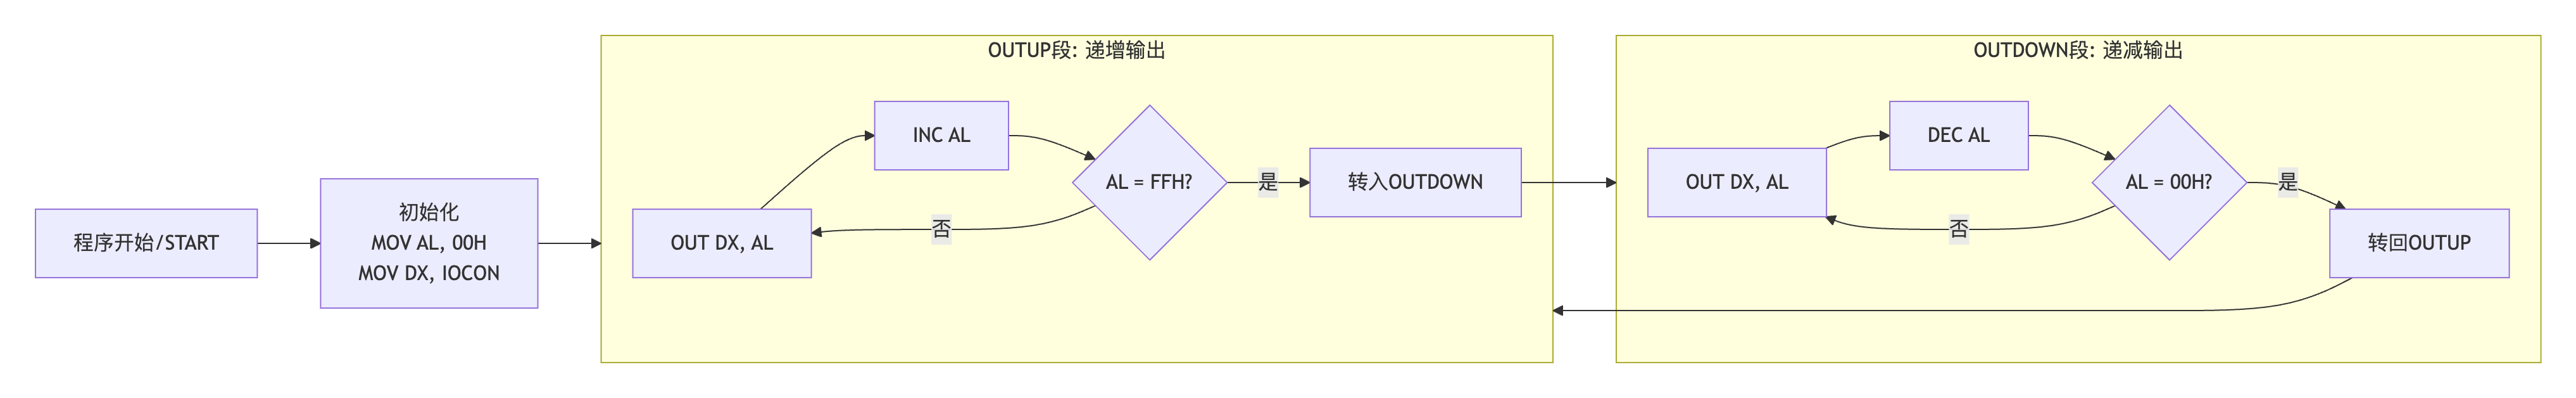
\includegraphics[width=\textwidth]{images/image-2025-12-15-14-24-07.png}
  \caption{三角波生成逻辑流程图}
  \label{fig:image-2025-12-15-14-24-07.png}
\end{figure}

\begin{lstlisting}[language={[x86masm]Assembler}]
    CODE SEGMENT
    ASSUME CS:CODE
    IOCON EQU 0B000H       

START:
    MOV AL, 00H           
    MOV DX, IOCON         

OUTUP:
    OUT DX, AL            
    INC AL                
    CMP AL, 0FFH          ; 判断是否达到最大值
    JE OUTDOWN            ; 达到则跳转递减段
    JMP OUTUP             

OUTDOWN:
    DEC AL                
    OUT DX, AL            
    CMP AL, 00H           ; 判断是否减到0
    JE OUTUP              ; 为0则跳回递增段
    JMP OUTDOWN           

CODE ENDS
END START
\end{lstlisting}

\subsubsection{锯齿波生成实验}

\begin{figure}[htbp]
  \centering
  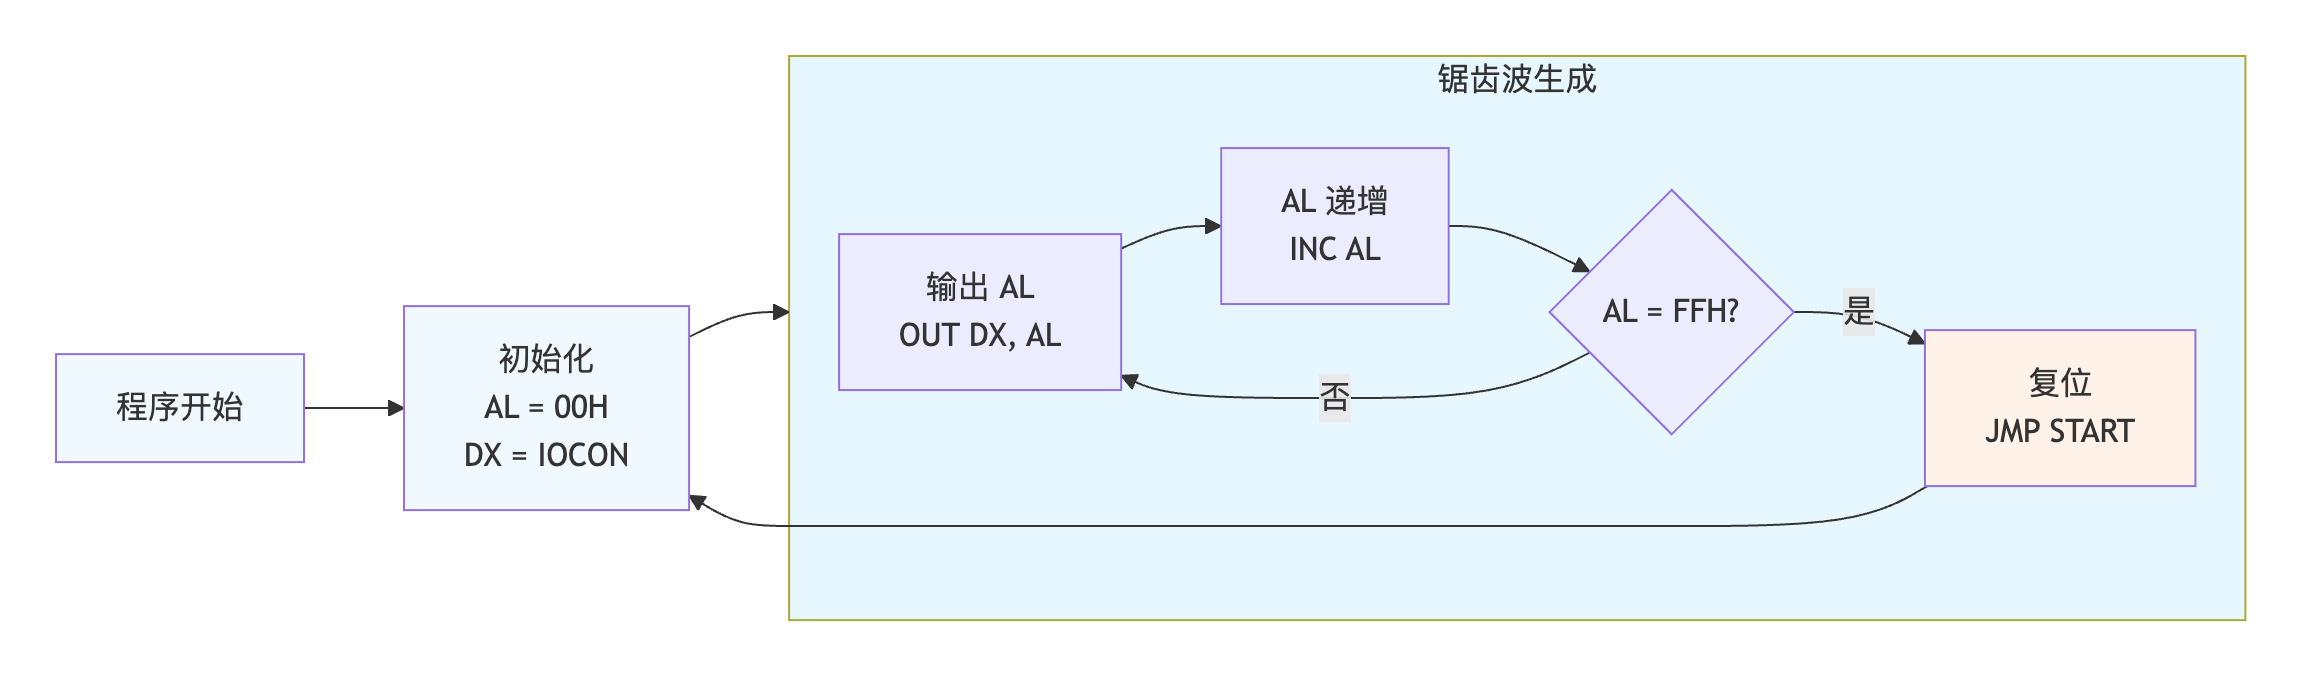
\includegraphics[width=\textwidth]{images/image-2025-12-15-14-26-50.png}
  \caption{锯齿波生成逻辑流程图}
  \label{fig:image-2025-12-15-14-26-50.png}
\end{figure}

\begin{lstlisting}[language={[x86masm]Assembler}]
    CODE SEGMENT
    ASSUME CS:CODE
    IOCON EQU 0B000H

START:
    MOV AL, 00H
    MOV DX, IOCON

OUTUP:
    OUT DX, AL
    INC AL
    CMP AL, 0FFH
    JE RESET
    JMP OUTUP

RESET:
    JMP START

CODE ENDS
END START
\end{lstlisting}

\subsubsection{正弦波生成实验}

\begin{figure}[htbp]
  \centering
  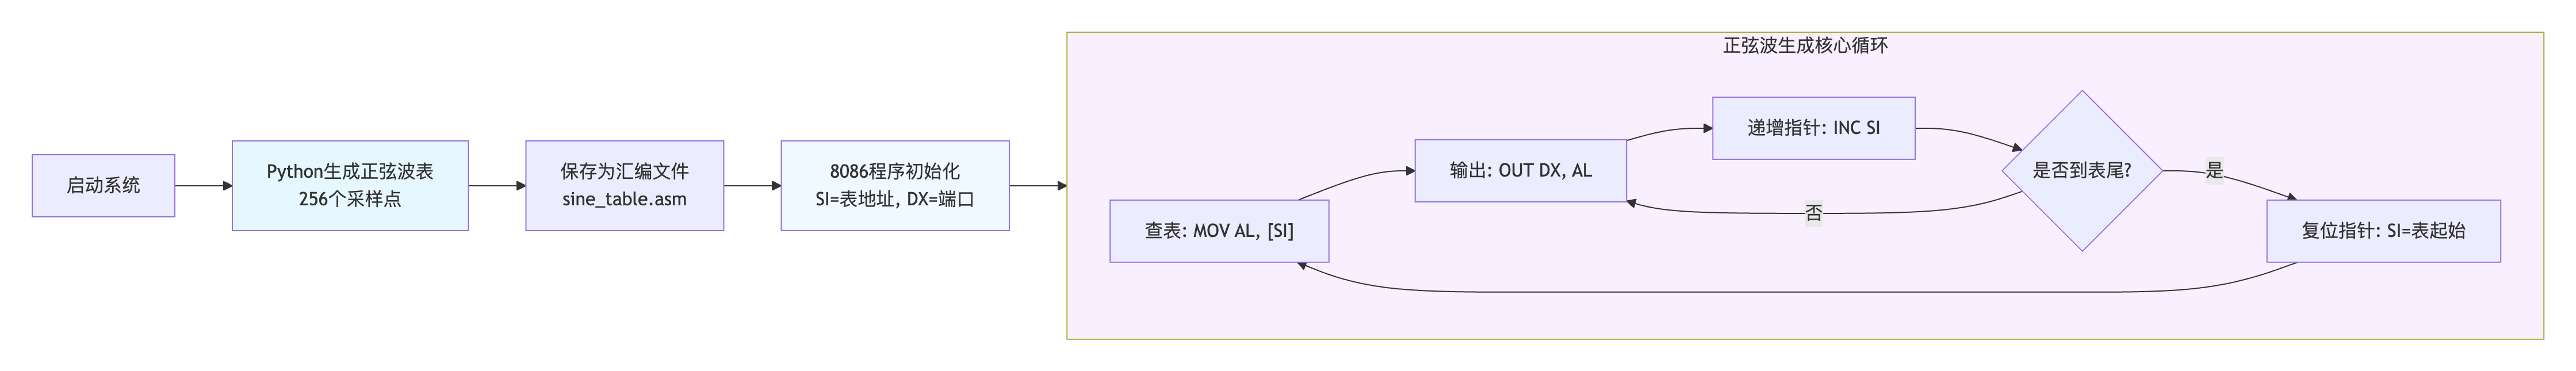
\includegraphics[width=\textwidth]{images/image-2025-12-15-14-46-29.png}
  \caption{正弦波生成逻辑流程图}
  \label{fig:image-2025-12-15-14-46-29.png}
\end{figure}

\textbf{第一步：生成正弦波数据表}

\begin{lstlisting}[language=bash]
    python sin_wave_generator.py
\end{lstlisting}

脚本代码见附录 A。

\textbf{第二步：根据正弦数据表生成正弦波}

\begin{lstlisting}[language={[x86masm]Assembler}]
CODE SEGMENT
    ASSUME CS:CODE, DS:DATA

START:
    MOV AX, DATA
    MOV DS, AX
    MOV SI, OFFSET SINE_TABLE
    MOV DX, IOCON
    
SINE_LOOP:
    MOV AL, [SI]               ; 查表获取正弦值
    OUT DX, AL                 ; 输出到端口
    
    INC SI                     ; 指针递增
    CMP SI, OFFSET SINE_TABLE_END
    JB CONTINUE                ; 未到表尾则继续
    MOV SI, OFFSET SINE_TABLE  ; 重置指针
    
CONTINUE:
    JMP SINE_LOOP

CODE ENDS

; 正弦波表（替换成Python脚本生成的版本）
DATA SEGMENT
SINE_TABLE DB 128, 131, 134, 137, 140, 143, 146, 149
           DB 152, 155, 158, 161, 164, 167, 170, 173
           ; ... 省略中间240个数据
           DB 125, 122, 119, 116, 113, 110, 107, 104
           DB 101, 98, 95, 92, 89, 86, 83, 80
SINE_TABLE_END LABEL BYTE
DATA ENDS
END START
\end{lstlisting}

\subsection{A/D 模数转换实验}

\begin{figure}[htbp]
  \centering
  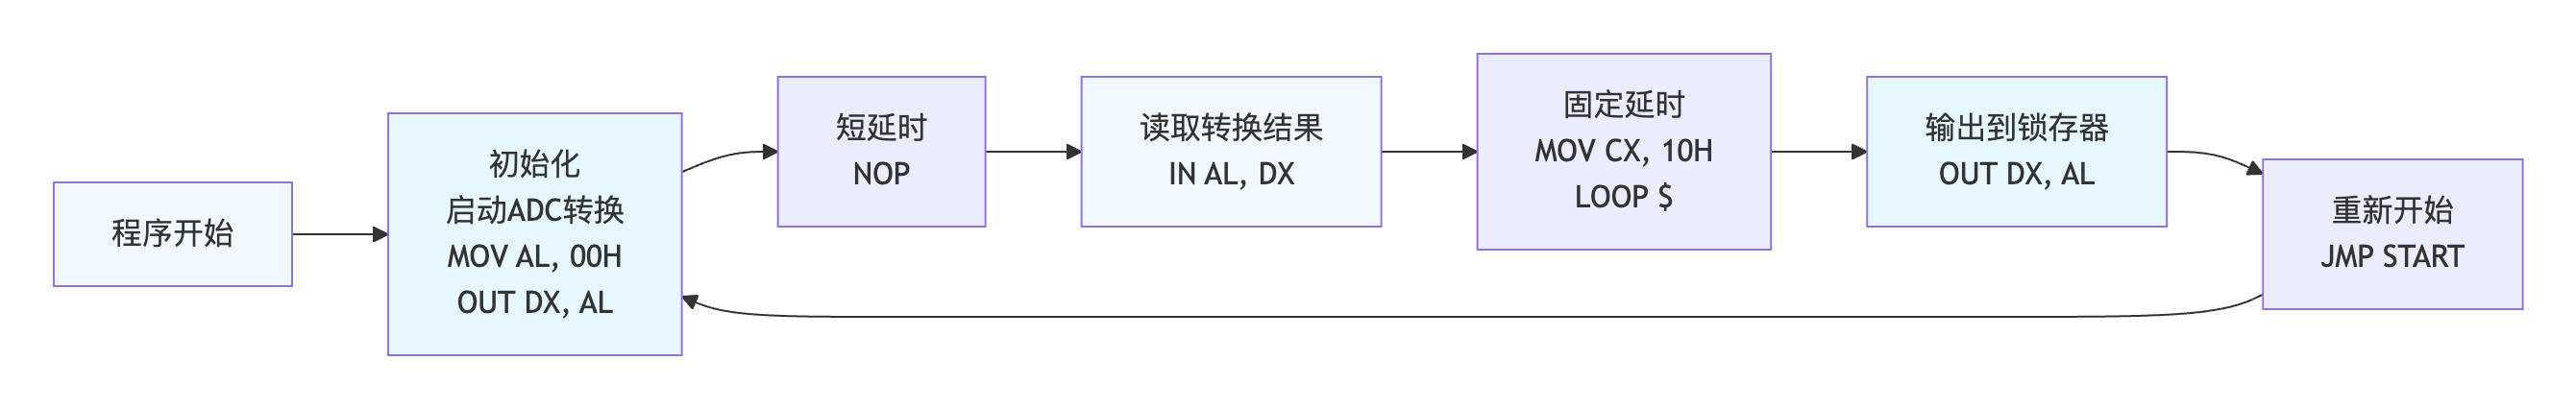
\includegraphics[width=0.8\textwidth]{images/image-2025-12-15-14-49-49.png}
  \caption{A/D 模数转换实验逻辑流程图}
  \label{fig:image-2025-12-15-14-49-49.png}
\end{figure}

\begin{lstlisting}[language={[x86masm]Assembler}]
CODE SEGMENT
    ASSUME CS:CODE
    
    AD0809 EQU 0E002H
    OUT373 EQU 8000H

START:
    MOV AL, 00H
    MOV DX, AD0809
    OUT DX, AL          ; 启动ADC0809转换
    
    NOP
    
    IN  AL, DX          ; 读取ADC0809转换结果
    MOV CX, 10H
    LOOP $              ; 延时等待
    MOV DX, OUT373
    OUT DX, AL          ; 结果输出到74LS373锁存器
    
    JMP START           ; 重新启动下一次转换

CODE ENDS
END START
\end{lstlisting}

\section{实验结果}

\subsection{D/A 数模转换实验}

\begin{figure}[htbp]
    \centering
    \begin{subfigure}{0.48\textwidth}
        \centering
        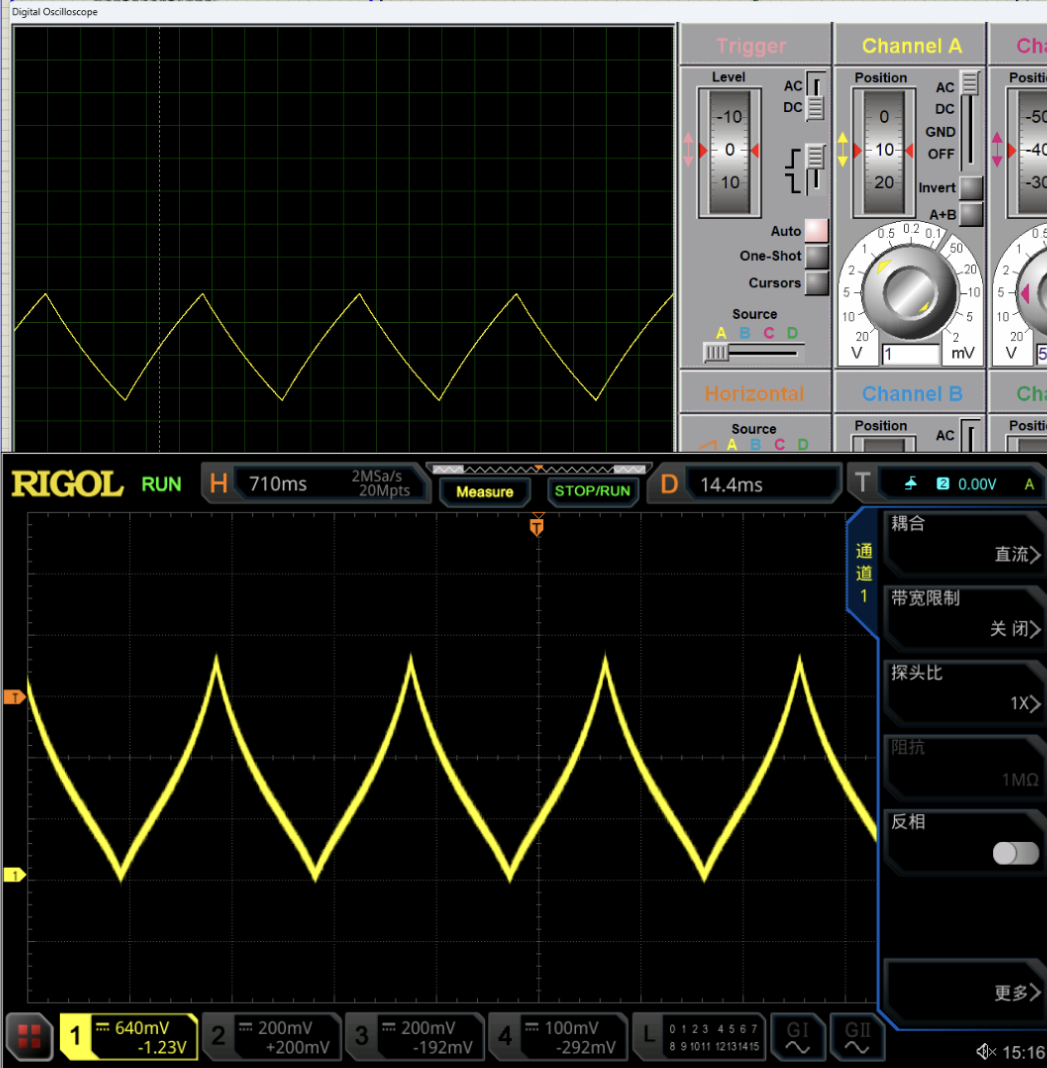
\includegraphics[width=\linewidth]{images/image-2025-12-15-14-51-28.png}
        \caption{三角波仿真软件-示波器截图}
        \label{fig:image-2025-12-15-14-51-28.png}
    \end{subfigure}
    \hfill
    \begin{subfigure}{0.48\textwidth}
        \centering
        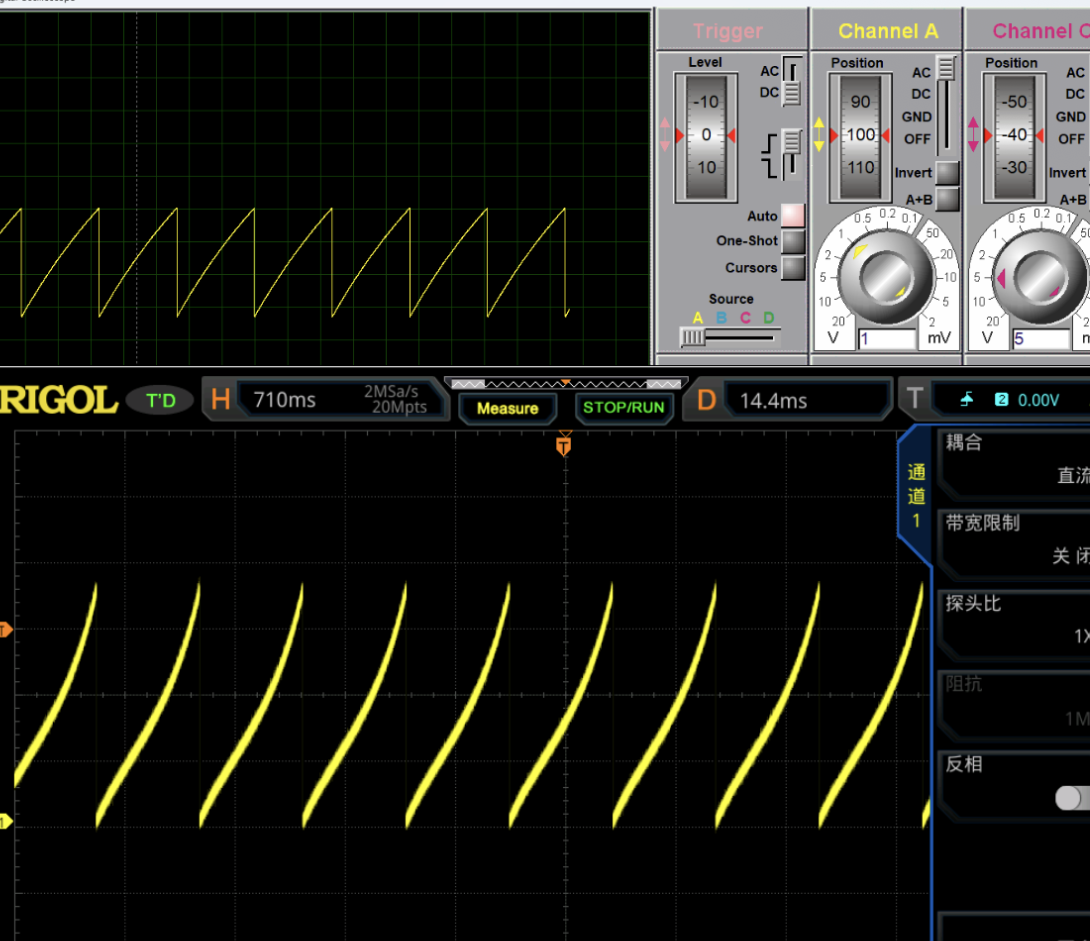
\includegraphics[width=\linewidth]{images/image-2025-12-15-14-52-47.png}
        \caption{锯齿波仿真软件-示波器截图}
        \label{fig:image-2025-12-15-14-52-47.png}
    \end{subfigure}
\end{figure}

\begin{figure}[htbp]
    \centering
    \begin{subfigure}{0.48\textwidth}
        \centering
        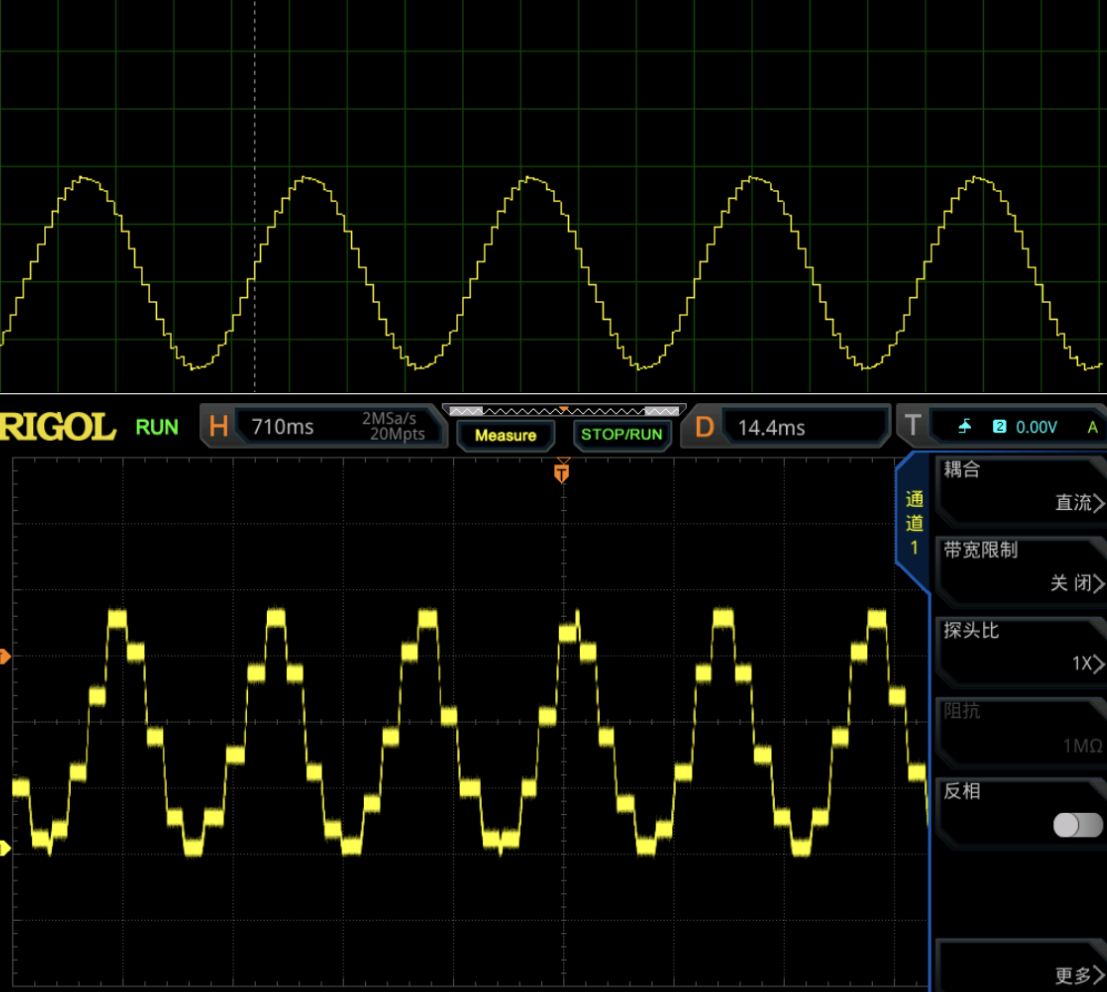
\includegraphics[width=\linewidth]{images/image-2025-12-15-14-53-20.png}
        \caption{正弦波（60 点拟合）仿真软件-示波器截图}
        \label{fig:image-2025-12-15-14-53-20.png}
    \end{subfigure}
    \hfill
    \begin{subfigure}{0.48\textwidth}
        \centering
        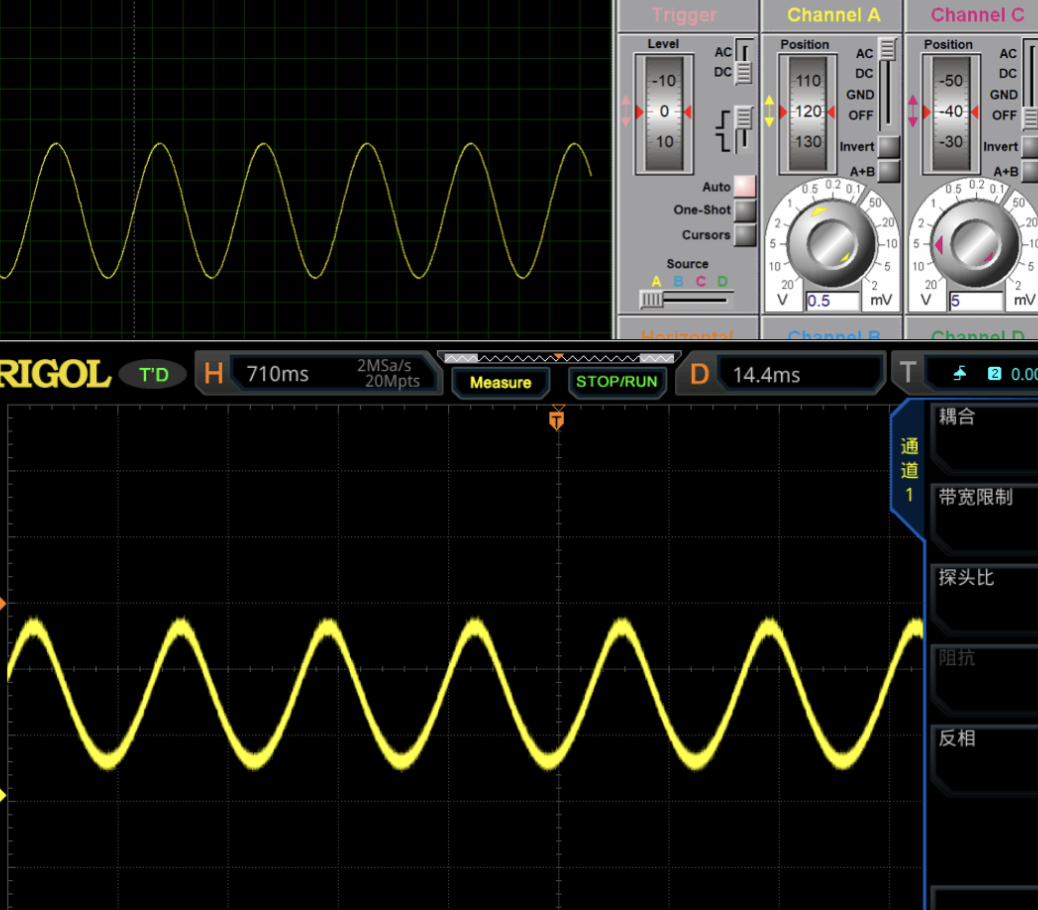
\includegraphics[width=\linewidth]{images/image-2025-12-15-14-54-43.png}
        \caption{正弦波（256 点拟合）仿真软件-示波器截图}
        \label{fig:image-2025-12-15-14-54-43.png}
    \end{subfigure}
\end{figure}

\vspace*{-3mm}
\begin{redbox}
    根据查表法与自动脚本配合，理论上可以生成任意精度的正弦波形状及其他函数波形，实际效果与数据点数量成正比。实验中发现，数据点数量越多，生成的正弦波形状越接近理想曲线，失真越小。
\end{redbox}

\subsection{A/D 模数转换实验}

\begin{figure}[H]
    \centering
    \begin{subfigure}{0.48\textwidth}
        \centering
        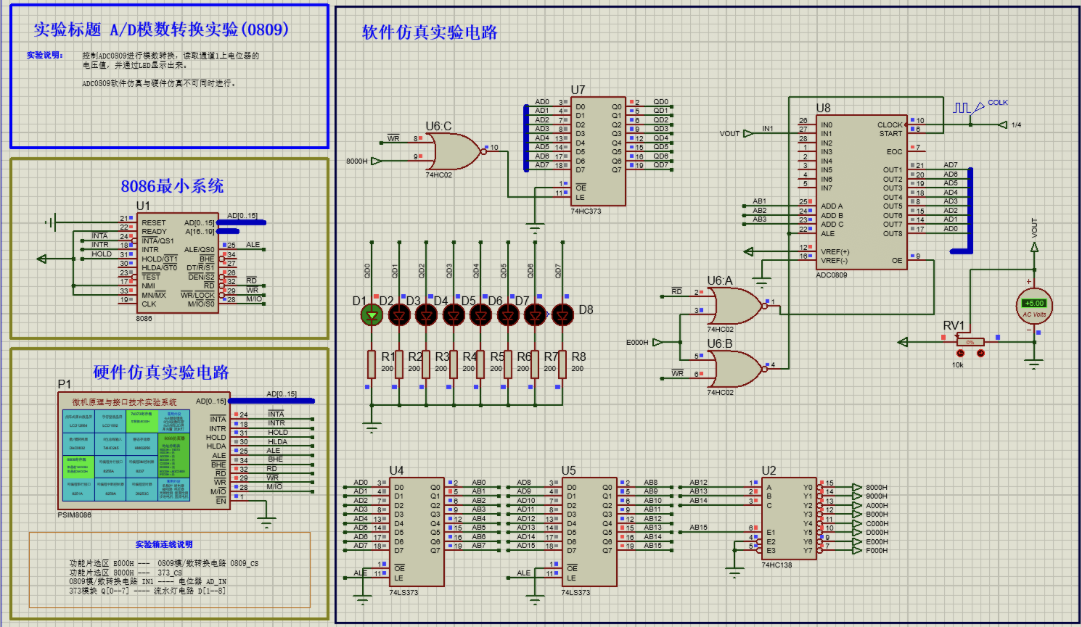
\includegraphics[width=\linewidth]{images/image-2025-12-15-14-57-34.png}
        \caption{电位器最小阻值仿真软件显示}
        \label{fig:image-2025-12-15-14-57-34.png}
    \end{subfigure}
    \hfill
    \begin{subfigure}{0.48\textwidth}
        \centering
        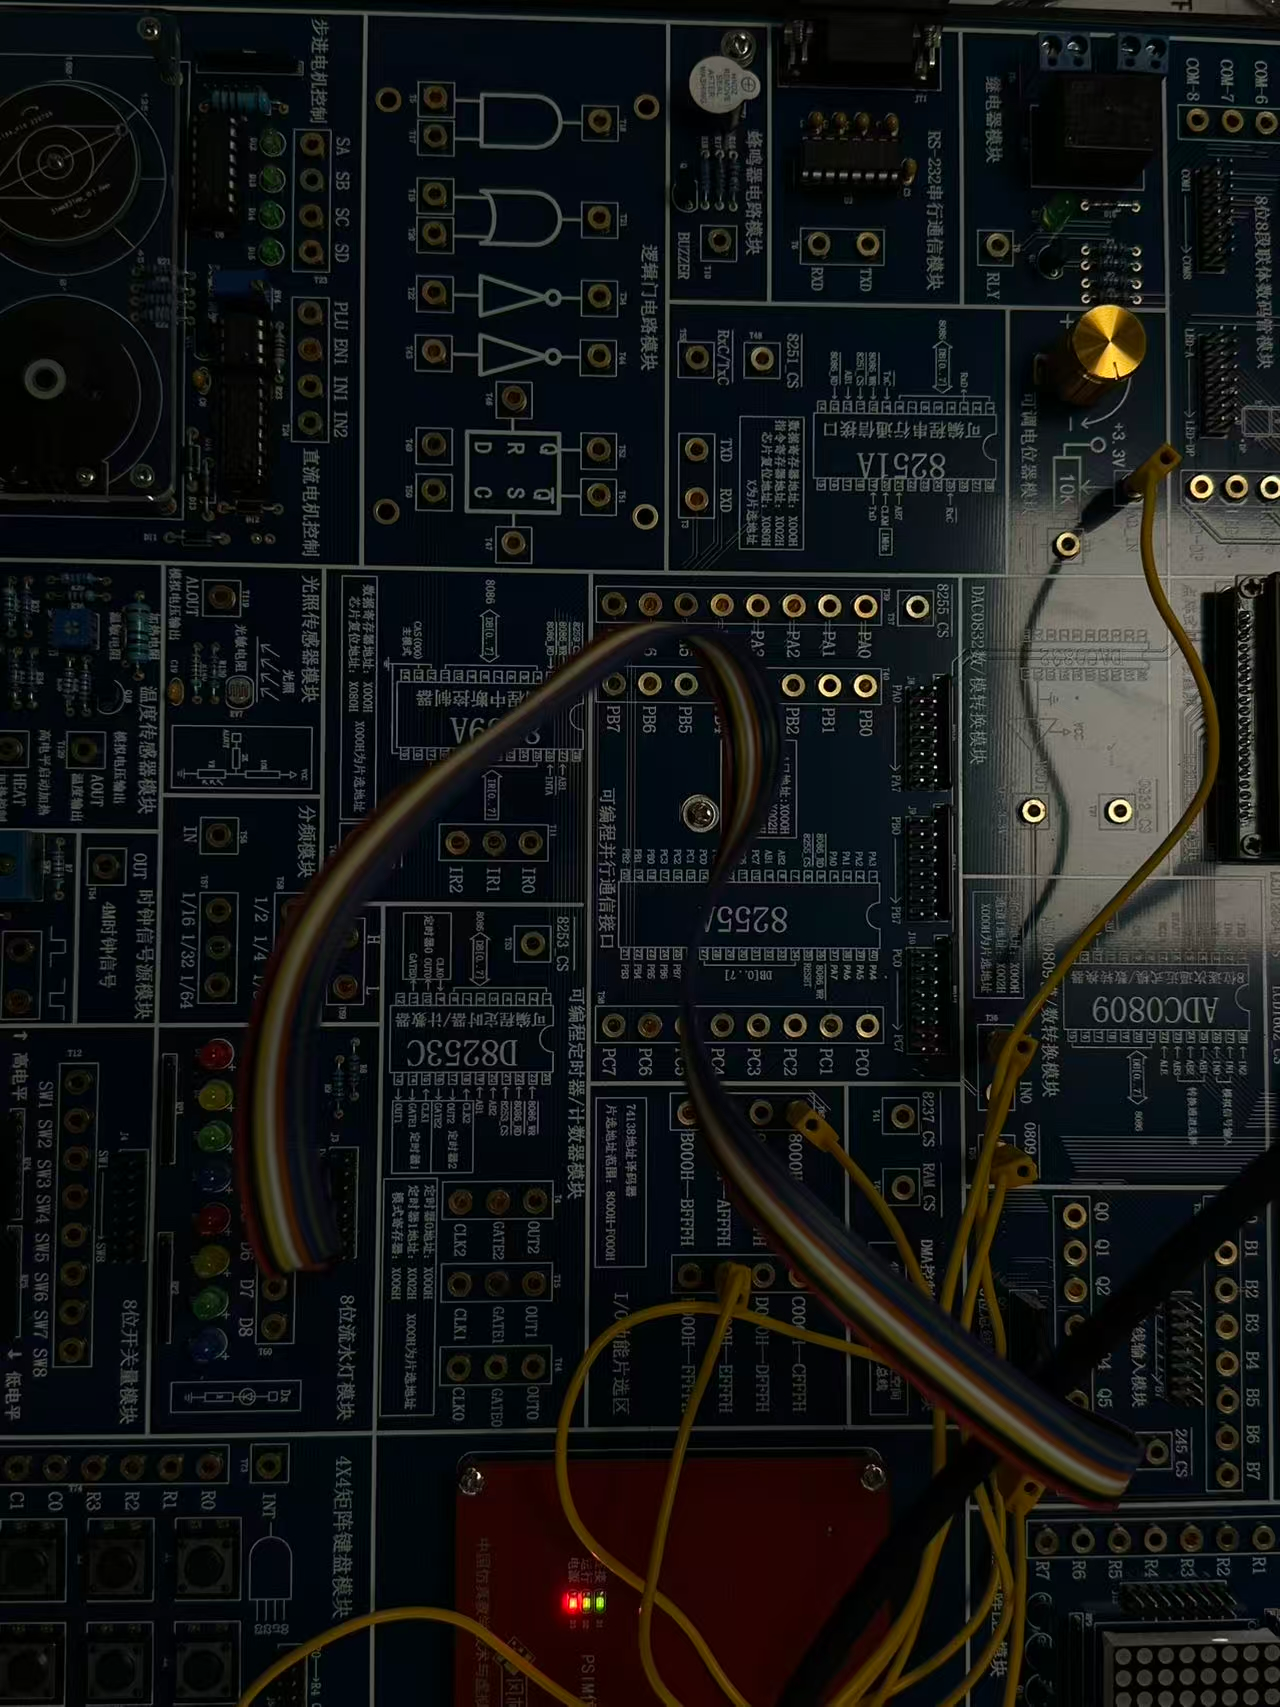
\includegraphics[width=\linewidth]{images/image-2025-12-15-15-04-05.png}
        \caption{电位器最小阻值LED灯珠显示}
        \label{fig:image-2025-12-15-15-04-05.png}
    \end{subfigure}
\end{figure}

\begin{figure}[H]
    \centering
    \begin{subfigure}{0.48\textwidth}
        \centering
        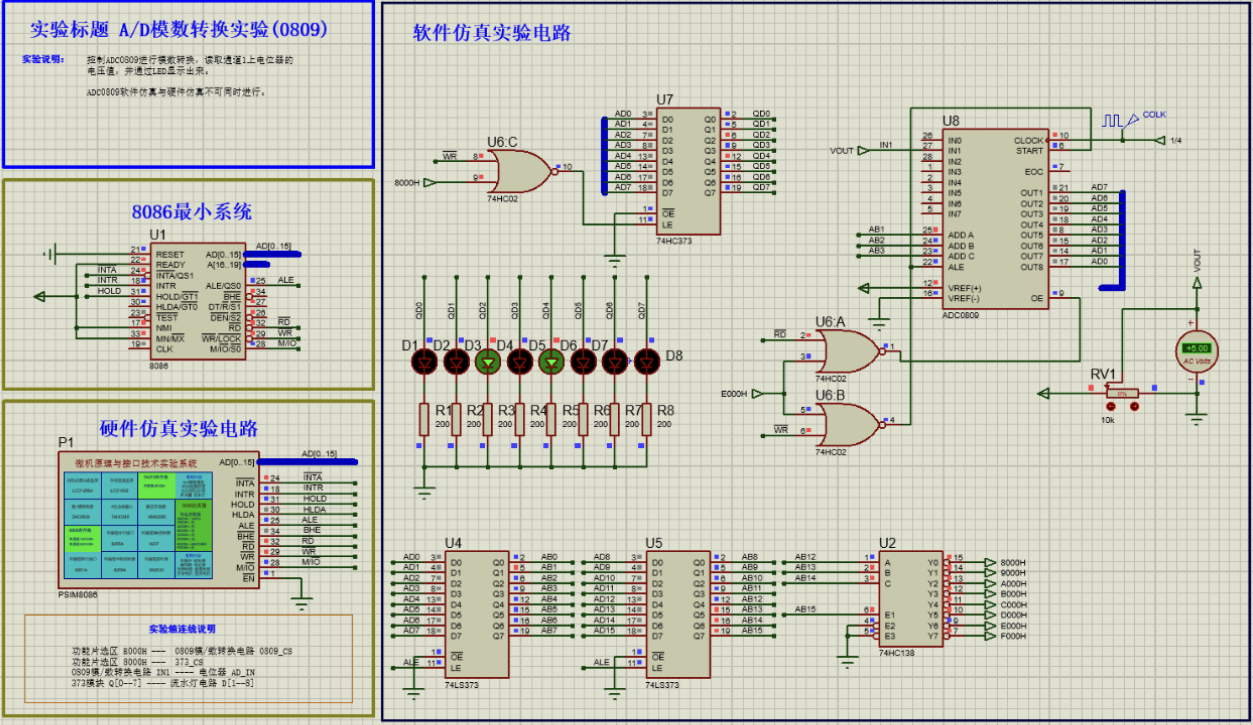
\includegraphics[width=\linewidth]{images/image-2025-12-15-15-11-26.png}
        \caption{电位器中间阻值时仿真软件显示}
        \label{fig:image-2025-12-15-15-11-26.png}
    \end{subfigure}
    \hfill
    \begin{subfigure}{0.48\textwidth}
        \centering
        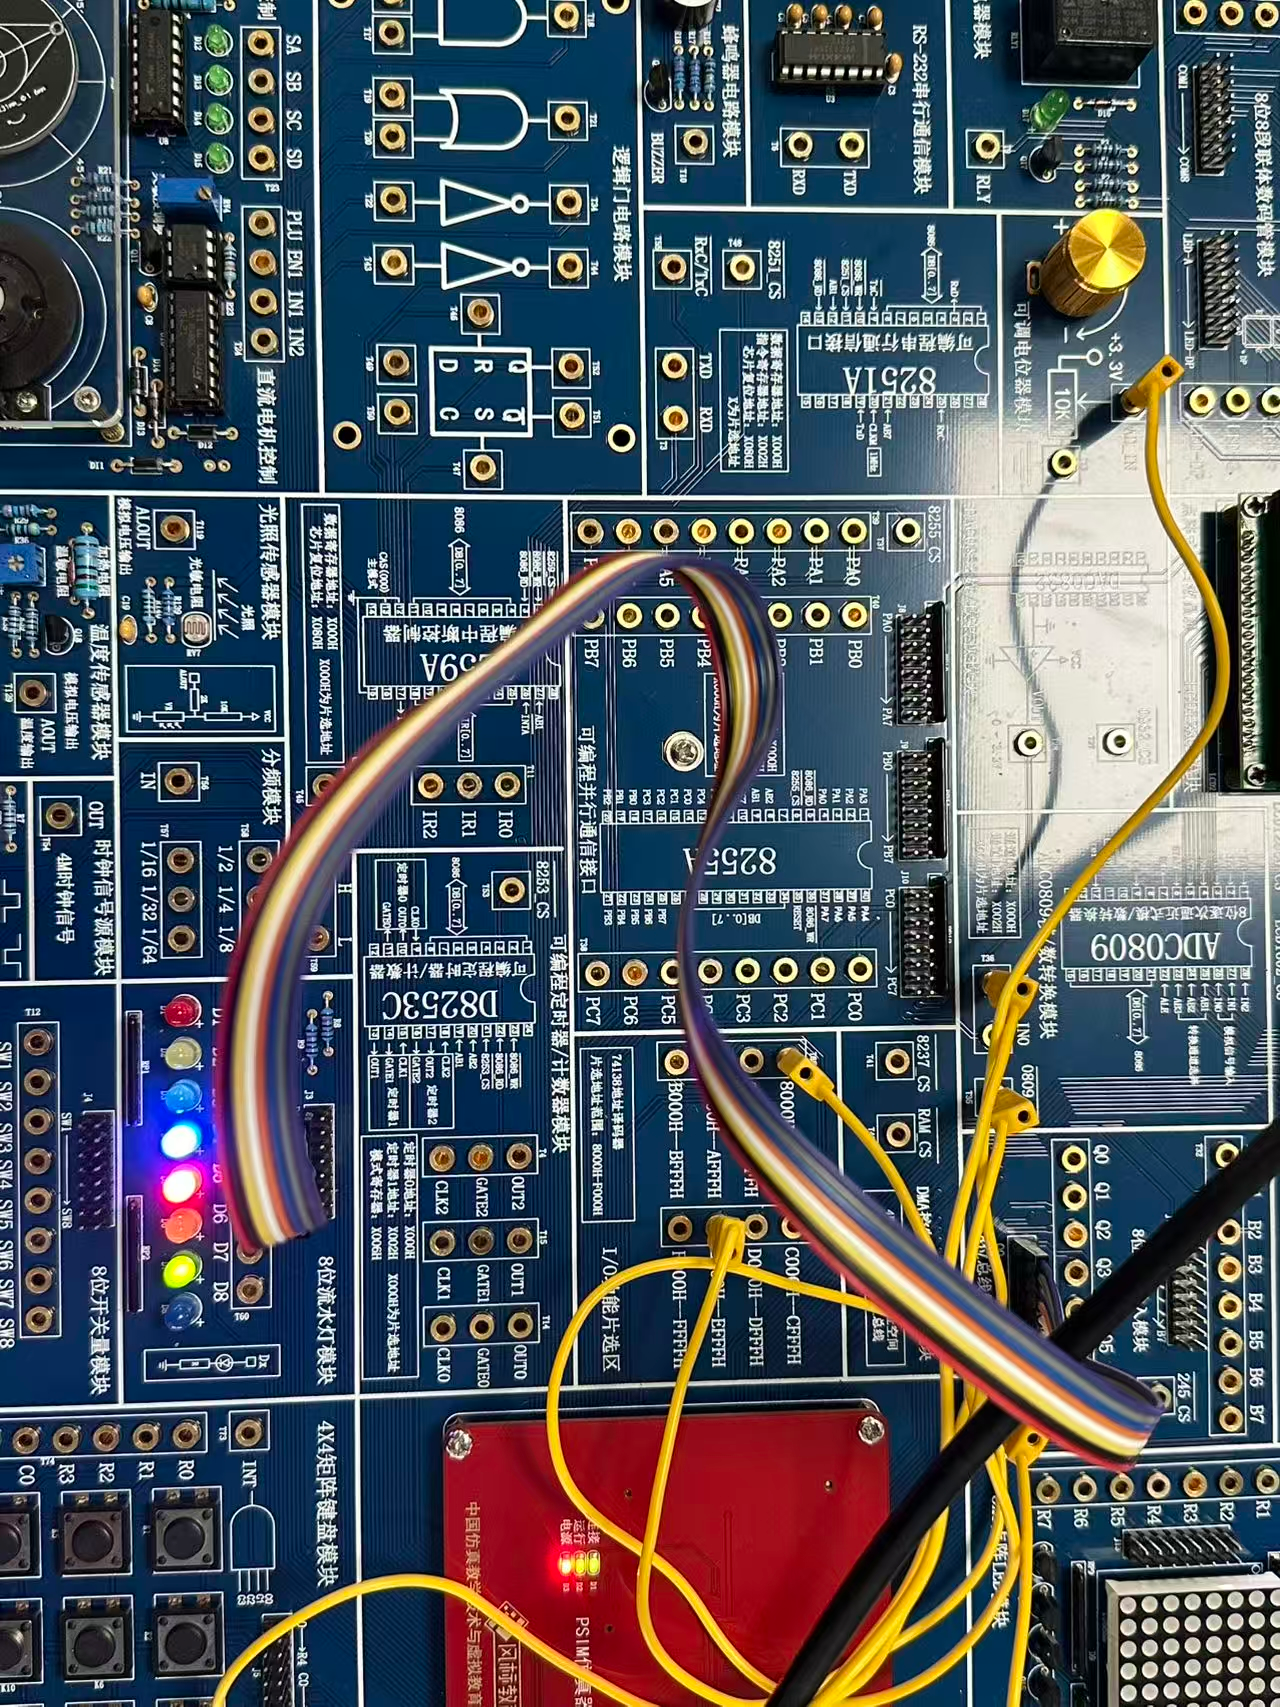
\includegraphics[width=\linewidth]{images/image-2025-12-15-15-10-12.png}
        \caption{电位器中间阻值时LED灯珠显示}
        \label{fig:image-2025-12-15-15-10-12.png}
    \end{subfigure}
\end{figure}

\section{思考与总结}

\subsection{关于 D/A 转换与波形拟合精度的思考}
    本次实验通过 D/A 转换器生成了三角波、锯齿波和正弦波。对于三角波和锯齿波，其生成逻辑是线性的，通过简单的寄存器加减指令即可实现。而对于正弦波，实验采用了\textbf{查表法}（Look-Up Table, LUT），这是一种典型的“以空间换时间”的算法策略。
    
    这两种策略在汇编层面的对比如下：

\begin{lstlisting}[language={[x86masm]Assembler}]
; 1. 线性生成 (锯齿波/三角波)
INC AL              ; 依赖 CPU 运算指令直接生成数据
OUT DX, AL          ; 实时性强，但波形单一

; 2. 查表法 (正弦波)
MOV AL, [SI]        ; 依赖预先计算好的内存数据
OUT DX, AL          ; 灵活性高，可生成任意波形
INC SI
\end{lstlisting}

    在实验中对比了 60 点拟合与 256 点拟合的效果，可以明显观察到点数越多，波形越平滑。这引出了 D/A 转换中的两个关键指标：\textbf{分辨率}和\textbf{采样率}。
    \begin{itemize}
        \item \textbf{幅度量化误差}：受限于 DAC0832 的 8 位精度，输出电压只能在 $0 \sim V_{ref}$ 之间分为 256 个离散电平，这导致波形在纵轴上必然存在锯齿状的量化噪声。
        \item \textbf{时间离散化}：CPU 输出数据的速度决定了横轴的时间分辨率。
    \end{itemize}
    \textbf{拓展思考}：在实际工程应用中，为了获得更纯净的模拟信号，通常会在 DAC 输出端级联一个\textbf{低通滤波器（LPF）}，用于滤除由阶梯波产生的高频谐波分量。

\subsection{关于 A/D 转换控制方式的改进探讨}
    在 A/D 模数转换实验中，代码使用了软件延时的方式来等待 ADC0809 完成转换。这种方式被称为\textbf{盲延时}，其缺点是 CPU 效率低下且依赖经验值。
    
    \textbf{改进方案}：利用 ADC0809 的 \textbf{EOC (End of Conversion)} 信号进行查询控制。相比于当前的延时代码，查询方式能自适应硬件速度：

\begin{lstlisting}[language={[x86masm]Assembler}]
; 当前方式：盲延时 (效率低)
MOV CX, 10H
LOOP $              ; CPU 空转等待

; 改进方式：查询 EOC 状态 (假设状态口为 STATUS_PORT)
WAIT_EOC:
    IN  AL, STATUS_PORT
    TEST AL, 80H    ; 检测 EOC 标志位 (假设在最高位)
    JZ  WAIT_EOC    ; 若未完成则继续等待
    IN  AL, DATA_PORT ; 完成后立即读取
\end{lstlisting}

    此外，更高级的控制方式是\textbf{中断方式}：将 EOC 信号连接至 CPU 的中断请求引脚（如 8259A 的 IRQ），转换结束后触发中断服务程序读取数据。这种方式下 CPU 利用率最高，适合多任务实时系统。

\subsection{微机接口实验的综合体会}
    通过本次实验，深刻理解了“端口”在微机系统中的核心地位。`OUT` 和 `IN` 指令不仅仅是数据的传输，往往还伴随着硬件控制信号的触发。
    
    例如，向 ADC0809 的通道地址写入数据这一操作：
\begin{lstlisting}[language={[x86masm]Assembler}]
OUT DX, AL  ; 既传输了通道号(AL)，又产生了 WR 写信号启动了转换
\end{lstlisting}
    这说明在接口技术中，软件指令与硬件时序是紧密耦合的。这种从“数字代码”到“模拟物理量”再回到“数字显示”的闭环过程，是微机原理与接口技术的精髓所在。

% \subsection*{4.1 \ \ }
% \subsection*{4.2 \ \ }
% \subsection*{4.3 \ \ }
% \subsection*{4.4 \ \ }
% \subsection*{4.5 \ \ }
% \subsection*{4.6 \ \ }




















































\newpage
% 附录
\section*{附录 A\hspace*{20pt} 脚本代码}
\addcontentsline{toc}{section}{附录 A\hspace*{6pt} 脚本代码} 
\thispagestyle{fancy} 

\begin{lstlisting}[language=Python]
import math

def generate_sine_table(num_points=256, amplitude=127.5, offset=127.5):
    sine_table = []
    for i in range(num_points):
        sine_value = math.sin(2 * math.pi * i / num_points)
        dac_value = int(amplitude * sine_value + offset)
        dac_value = max(0, min(255, dac_value))
        sine_table.append(dac_value)
    return sine_table

def save_as_assembly_table(sine_table, filename="sine_table.asm"):
    with open(filename, 'w') as f:
        f.write("SINE_TABLE LABEL BYTE\n")
        for i, value in enumerate(sine_table):
            if i % 16 == 0:
                f.write(f"\tDB {value}")
            else:
                f.write(f", {value}")
            if i % 16 == 15 or i == len(sine_table) - 1:
                f.write("\n")

def main():
    sine_table = generate_sine_table()
    save_as_assembly_table(sine_table)
    print(f"表大小: {len(sine_table)} 字节")
    print("前10个正弦波值:")
    for i in range(10):
        print(f"位置 {i}: {sine_table[i]} (0x{sine_table[i]:02X})")
    print(f"最小值: {min(sine_table)}")
    print(f"最大值: {max(sine_table)}")
    print(f"平均值: {sum(sine_table)/len(sine_table):.1f}")

if __name__ == "__main__":
    main()
\end{lstlisting}



\end{document}

% VScode 常用快捷键：

% F2:                       变量重命名
% Ctrl + Enter:             行中换行
% Alt + up/down:            上下移行
% 鼠标中键 + 移动:           快速多光标
% Shift + Alt + up/down:    上下复制
% Ctrl + left/right:        左右跳单词
% Ctrl + Backspace/Delete:  左右删单词    
% Shift + Delete:           删除此行
% Ctrl + J:                 打开 VScode 下栏(输出栏)
% Ctrl + B:                 打开 VScode 左栏(目录栏)
% Ctrl + `:                 打开 VScode 终端栏
% Ctrl + 0:                 定位文件
% Ctrl + Tab:               切换已打开的文件(切标签)
% Ctrl + Shift + P:         打开全局命令(设置)

% Latex 常用快捷键：

% Ctrl + Alt + J:           由代码定位到PDF


